\newpage
%\end{multicols*}
\section{Zeitdiskrete Systeme}
\subsection{Elementare, zeitdiskrete Signale}
	\begin{itemize}[leftmargin=*]
		\item \textbf{Einheitsimpuls}, Impulsfolge, Delta-Impuls $\delta(n)$\\
		      \makebox[\columnwidth][c]
		      {
			      \begin{minipage}{0.3\columnwidth}
				      \[ \boxed{
					      \delta(n) =
					      \begin{cases}
						      1 & n = 0    \\
						      0 & n \neq 0
					      \end{cases}
					    }
				      \]
			      \end{minipage}
			      \begin{minipage}{0.7\columnwidth}
				      \centering
				      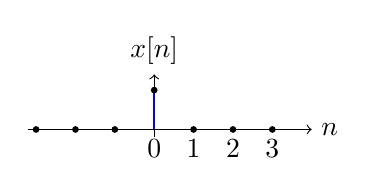
\begin{tikzpicture}[baseline=0.8,scale=0.5]
					      \draw[->] (0,-0.2) -- (0,1.4) node[above]{$x[n]$}; %y
					      \draw[->] (-3.2,0) -- (4,0) node[right]{$n$}; %x
					      \filldraw[black] (-3,0) circle (2pt) {};
					      \filldraw[black] (-2,0) circle (2pt) {};
					      \filldraw[black] (-1,0) circle (2pt) {};
					      \draw[blue, thick] (0,1) -- (0,0) node[below, black]{0}; \filldraw[black] (0,1) circle (2pt) {};
					      \filldraw[black] (1,0) circle (2pt) node[below]{1};
					      \filldraw[black] (2,0) circle (2pt) node[below]{2};
					      \filldraw[black] (3,0) circle (2pt) node[below]{3};
				      \end{tikzpicture}
			      \end{minipage}
		      }\\
		      
		      Eigenschaften:
		      \begin{itemize}
		      	  \item Zusammenhang mit Einheitssprung:
		      	  $$\sum^{\infty}_{n=-\infty}\delta(n)=1 \qquad \boxed{ \varepsilon(n)=\sum_{k=-\infty}^{n} \delta(n) } $$
			      \item Anregung der Impulsantwort
			      \item konstantes Spektrum
			      \item Ausblendeigenschaft:
			      \[
			      x(n) = \sum_{k=-\infty}^{\infty} x(k)\cdot\delta(n-k)
			      \]
		      \end{itemize}

		\item \textbf{Einheitssprung}\\
		      \makebox[\columnwidth][c]
		      {
			      \begin{minipage}{0.3\columnwidth}
				      \[
					      \varepsilon(n) =
					      \begin{cases}
						      1 & n \geq 0 \\
						      0 & n < 0
					      \end{cases}
				      \]
			      \end{minipage}
			      \begin{minipage}{0.7\columnwidth}
				      \centering
				      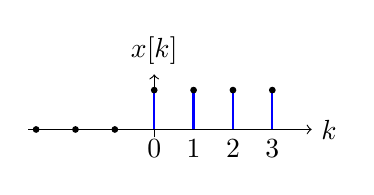
\begin{tikzpicture}[baseline=0.8,scale=0.5]
					      \draw[->] (0,-0.2) -- (0,1.4) node[above]{$x[k]$}; %y
					      \draw[->] (-3.2,0) -- (4,0) node[right]{$k$}; %x
					      \filldraw[black] (-3,0) circle (2pt) {};
					      \filldraw[black] (-2,0) circle (2pt) {};
					      \filldraw[black] (-1,0) circle (2pt) {};
					      \draw[blue, thick] (0,1) -- (0,0) node[below, black]{0}; \filldraw[black] (0,1) circle (2pt) {};
					      \draw[blue, thick] (1,1) -- (1,0) node[below, black]{1}; \filldraw[black] (1,1) circle (2pt) {};
					      \draw[blue, thick] (2,1) -- (2,0) node[below, black]{2}; \filldraw[black] (2,1) circle (2pt) {};
					      \draw[blue, thick] (3,1) -- (3,0) node[below, black]{3}; \filldraw[black] (3,1) circle (2pt) {};
				      \end{tikzpicture}
			      \end{minipage}
		      }
		      Zusammenhang mit Einheitsimpuls:
		      \[ \boxed{
			      \delta(n) = \varepsilon(n) - \varepsilon(n-1) }
		      \]
		\item \textbf{Rechteckfolge}\\
		      \makebox[\columnwidth][c]
		      {
			      \begin{minipage}{0.3\columnwidth}
				      \[
					      \operatorname{rect}_N(n) =
					      \begin{cases}
						      1 & 0 \leq n < N   \\
						      0 & \texttt{sonst}
					      \end{cases}
				      \]
			      \end{minipage}
			      \begin{minipage}{0.7\columnwidth}
				      \centering
				      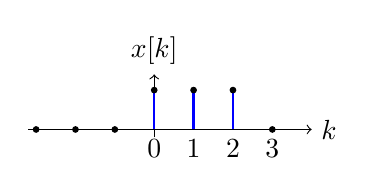
\begin{tikzpicture}[baseline=0.8,scale=0.5]
					      \draw[->] (0,-0.2) -- (0,1.4) node[above]{$x[k]$}; %y
					      \draw[->] (-3.2,0) -- (4,0) node[right]{$k$}; %x
					      \filldraw[black] (-3,0) circle (2pt) {};
					      \filldraw[black] (-2,0) circle (2pt) {};
					      \filldraw[black] (-1,0) circle (2pt) {};
					      \draw[blue, thick] (0,1) -- (0,0) node[below, black]{0}; \filldraw[black] (0,1) circle (2pt) {};
					      \draw[blue, thick] (1,1) -- (1,0) node[below, black]{1}; \filldraw[black] (1,1) circle (2pt) {};
					      \draw[blue, thick] (2,1) -- (2,0) node[below, black]{2}; \filldraw[black] (2,1) circle (2pt) {};
					      \filldraw[black] (3,0) circle (2pt) node[below] {3};
				      \end{tikzpicture}
			      \end{minipage}
		      }
		      Zusammenhang mit Einheitsimpuls bzw. -sprung:
		      \begin{align*}
			      \operatorname{rect}(n) & = \varepsilon(n) + \varepsilon(n-N)       \\
			                             & = \varepsilon(n) \cdot \varepsilon(N-1-n)
			                             \\
			                             & = \sum_{k=0}^{N-1} \delta(n-k)
		      \end{align*}
		\item \textbf{Zeitdiskreter Sinus}\\
		      \makebox[\columnwidth][c]
		      {
			      \begin{minipage}{0.3\columnwidth}
				      \[
					      x(n) = A \cdot \sin(\Omega\, n+\varphi)
				      \]
				      \small
				      
				      $A$       : Amplitude            \\
				      $\Omega$  : normierte\\ Kreisfrequenz \\
				      $\varphi$ : Anfangsphase
				      
				      \normalsize
				      
%  		      \begin{align*}
%				      	A       & :\texttt{Amplitude}               \\
%				      	\Omega  & :\texttt{normierte Kreisfrequenz} \\
%				      	\varphi & :\texttt{Anfangsphase}
%				\end{align*}
			      \end{minipage}
			      \begin{minipage}{0.7\columnwidth}
				      \centering
				      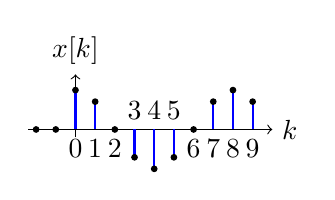
\begin{tikzpicture}[baseline=1,scale=0.5]
					      \draw[->] (0,-0.2) -- (0,1.4) node[above]{$x[k]$}; %y
					      \draw[->] (-1.2,0) -- (5,0) node[right]{$k$}; %x
					      \filldraw[black] (-1,0) circle (2pt) {};
					      \filldraw[black] (-0.5,0) circle (2pt) {};
					      \draw[blue,thick] (0,1) -- (0,0)          node[below, black]{0}; \filldraw[black] (0,1) circle (2pt) {};
					      \draw[blue,thick] (0.5,0.707) -- (0.5,0)  node[below, black]{1}; \filldraw[black] (0.5,0.707) circle (2pt) {};
					      \filldraw[black] (1,0) circle (2pt)              node[below, black]{2};
					      \draw[blue,thick] (1.5,-0.707) -- (1.5,0) node[above, black]{3}; \filldraw[black] (1.5,-0.707) circle (2pt) {};
					      \draw[blue,thick] (2,-1) -- (2,0)         node[above, black]{4}; \filldraw[black] (2,-1) circle (2pt) {};
					      \draw[blue,thick] (2.5,-0.707) -- (2.5,0) node[above, black]{5}; \filldraw[black] (2.5,-0.707) circle (2pt) {};
					      \filldraw[black] (3,0) circle (2pt)              node[below]{6};
					      \draw[blue,thick] (3.5,0.707) -- (3.5,0)  node[below, black]{7}; \filldraw[black] (3.5,0.707) circle (2pt) {};
					      \draw[blue,thick] (4,1) -- (4,0)          node[below, black]{8}; \filldraw[black] (4,1) circle (2pt) {};
					      \draw[blue,thick] (4.5,0.707) -- (4.5,0)  node[below, black]{9}; \filldraw[black] (4.5,0.707) circle (2pt) {};
				      \end{tikzpicture}
			      \end{minipage}
		      }

		\item \textbf{Komplexe Exponentialfolge}\\
		      \makebox[\columnwidth][c]
		      {
			      \begin{minipage}{0.3\columnwidth}
				      \begin{align*}
					      x(n) & = \underline{A} \cdot e^{Sn}                \\
					           & = \underline{A} \cdot e^{(\Sigma+j\Omega)n}
				      \end{align*}
			      \end{minipage}
			      \begin{minipage}{0.7\columnwidth}
				      \centering
				      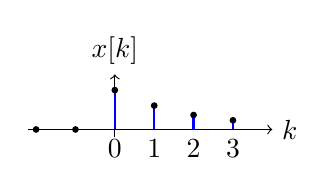
\begin{tikzpicture}[baseline=0.8,scale=0.5]
					      \draw[->] (0,-0.2) -- (0,1.4) node[above]{$x[k]$}; %y
					      \draw[->] (-2.2,0) -- (4,0) node[right]{$k$}; %x
					      \filldraw[black] (-2,0) circle (2pt) {};
					      \filldraw[black] (-1,0) circle (2pt) {};
					      \draw[blue, thick] (0,1) -- (0,0) node[below, black]{0}; \filldraw[black] (0,1) circle (2pt) {};
					      \draw[blue, thick] (1,0.606) -- (1,0) node[below, black]{1}; \filldraw[black] (1,0.606) circle (2pt) {};
					      \draw[blue, thick] (2,0.367) -- (2,0) node[below, black]{2}; \filldraw[black] (2,0.367) circle (2pt) {};
					      \draw[blue, thick] (3,0.233) -- (3,0) node[below, black]{3}; \filldraw[black] (3,0.233) circle (2pt) {};
				      \end{tikzpicture}
			      \end{minipage}
		      }
		      \begin{align*}
			      S                                       & = \Sigma+j\Omega        \\
			      \texttt{Amplitudenänderung }\Sigma      & = \sigma T = \sigma/f_A \\
			      \texttt{normierte Kreisfrequenz }\Omega & = \omega T =  2\pi \frac{f_0}{f_A}
		      \end{align*}
	\end{itemize}
%	\clearpage
%\begin{multicols*}{2}
\subsection{A/D-Wandlung}
\small
\begin{itemize}
	\item Zeitdiskretisierung, Abtastung, \textbf{Abtastrate}: $\boxed{f_a = \dfrac{1}{t_a}}$
	\[
	x(n)= x_0(t)\big|_{t = n{T_a}} = x_0 (nT) = x_0\left(\frac{n}{f_a}\right)
	\]
	\item Wertdiskretisierung (Quantisierung): Bitbreite, Aufl\"osung: 8 Bit = 256 Stufen.
	\item Abtastung Analog-Signal $\rightarrow$ \textbf{periodische} Fortsetzung des Analog-Spektrums im Abstand von $$ \boxed{
	\omega_a=\frac{2\pi}{t_a}=2\pi f_a \text{\qquad mit } t_a\text{: Abtastintervall} }$$
	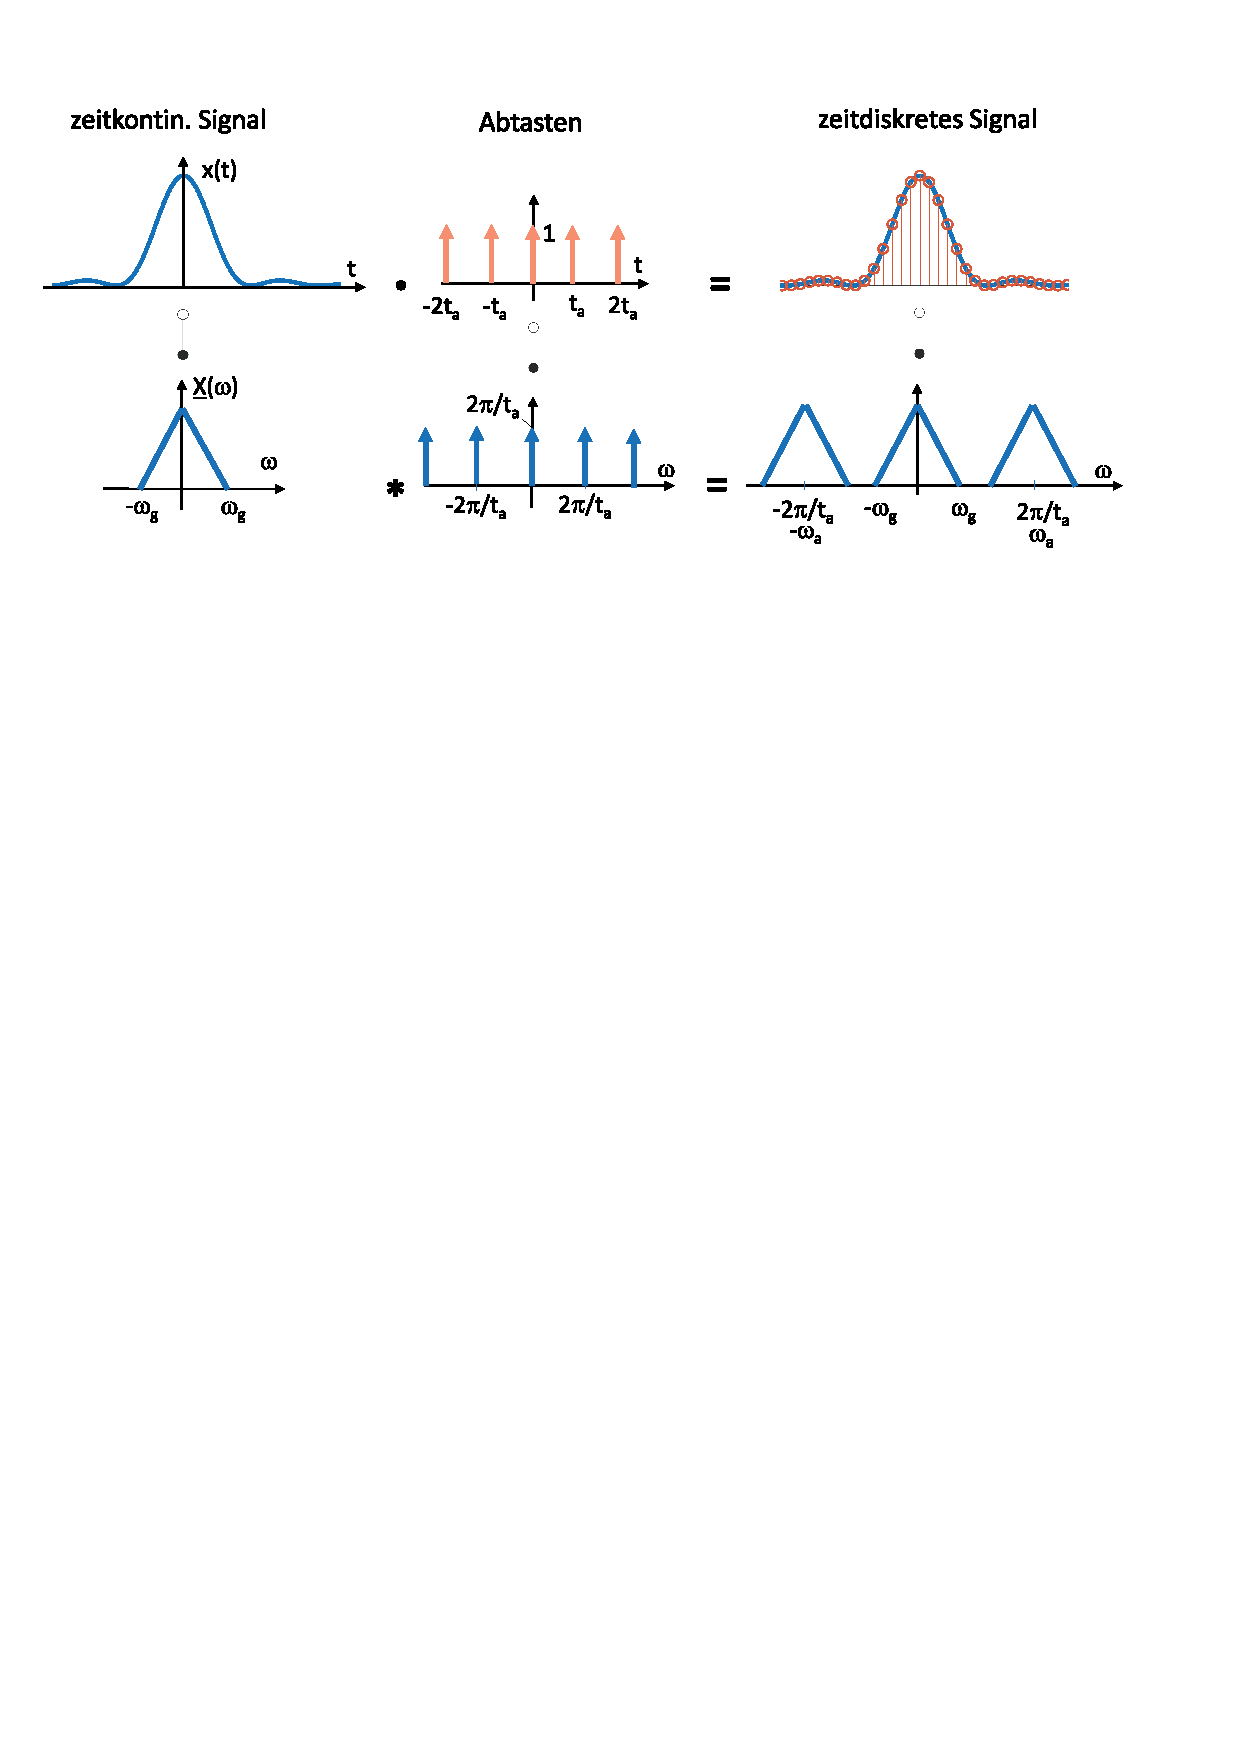
\includegraphics[width=0.9\columnwidth]{Bilder/Abtastung_Frequenzbereich_Spektrum_Original}
	\item \textbf{Aliasing}: {\small Spektrale \"Uberlagerung, zus\"atzliche Frequenzen/Abtastwerte, keine Rekonstruktion des Originalsignals aus $t_a=\frac{1}{f_a}$ m\"oglich.\\
				
	\textit{Abhilfe}: Eingangssignal auf $\omega_g$-Band begrenzen und\\ \textbf{Abtasttheorem} einhalten, Verringerung von $t_a$.}
\normalsize
\begin{gather*}
	\boxed{\omega_a \ge 2 \omega_g} \text{ bzw. } f_a \ge 2 f_g\\
	\boxed{\omega_g \le \frac{\omega_a}{2}} = \frac{1}{2} \cdot \frac{2\pi}{t_a} \text{ bzw. } f_g \ge \frac{f_a}{2}
\end{gather*}
%\begin{figure}[h!]
%	\centering
%	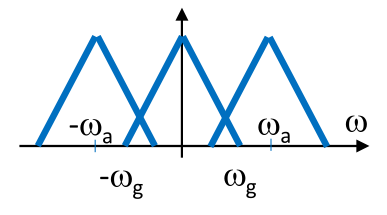
\includegraphics[width=\columnwidth]{Bilder/Abtasttheorem_Uebrlappung}
%\end{figure}
{\footnotesize Merke: zeitbegrenztes Signal: $\infty$ langes Spektrum $\rightarrow$ Aliasing\\
Dirac-Sprung im Signal: $\infty$ hohe $f$ im Spektrum $\rightarrow$ Aliasing}

\item Spektrum $U_a(\omega)$ eines abgetasteten Signals $u_a(t)$ mit $T=t_a = \frac{1}{f_a}$ aus einem Analogsignal $u(t)$:
\begin{align*}
U_a(\omega) &= 2\pi \cdot \sum_{k=-\infty}^{+\infty} \underline{c}_k \cdot \delta(\omega-k\omega_a)\\
& = 2\pi \cdot \sum_{k=-\infty}^{+\infty} \frac{\underline{U}(\omega)}{t_a} \cdot \delta(\omega-k\omega_a)\\
&= \frac{2\pi}{t_a} \cdot \sum_{k=-\infty}^{+\infty} \underline{U}(\omega) \cdot \delta(\omega-k\omega_a) \\
& =  \omega_a \cdot \sum_{k=-\infty}^{+\infty} \underline{U}(\omega-k\omega_a)
\end{align*}

\end{itemize}
\clearpage
\vspace{-1.5em}
\subsection{Zeitdiskrete LTI-Systeme}
\subsubsection{Systemeigenschaften}
\begin{itemize}
	\item \textbf{Linear}: System mit Ü-Fkt. $\underline{H}(z)$ beschreibbar.
	\item \textbf{Kausal}:
	      Anzahl der Pole (Grad des Nenners)  $N\ge M$\\
	      Anzahl der Nullstellen (Grad des Zählers),\\
	      $ h(n) = 0 \texttt{ für } n<0 $, rechtsseitige Folge.
	\item \textbf{Stabil}:
	      Einheitskreis (EK) $\in$ Konvergenzbereich (KB),\\
	   absolute Summierbarkeit: $ \sum_{n=-\infty}^{\infty}|h(n))| < \infty $,\\
	   \textbf{Alle} Pole $\in$ EK.
	\item \textbf{minimalphasiges} LTI-System: \textbf{Alle} Nullstellen $\in$ EK.
\end{itemize}


\subsubsection{Impuls- \& Systemantwort, Faltung}
\small
\begin{centering}
\begin{tabularx}{\columnwidth}{|X|X|}
	\hline
	Impulsanregung & Impulsantwort\\
	\hline
	$x(n)=\delta(n)$ & $y(n)= h(n) = S\{ \delta(n) \}$ \\
	\hline
	{
	\begin{align*}
		x(n) &= \sum_{k=-\infty}^{\infty}x(k) \cdot \delta(n-k)\\
		\delta(n) &= \varepsilon(n)-\varepsilon(n-1)
	\end{align*}
	}	 &
	{
	\begin{align*}	
		y(n) &= \sum_{k=-\infty}^{\infty}x(k) \cdot h(n-k)\\
		&= x(n) * h(n)\\
		h(n) &= g(n)-g(n-1)\\
		\underline{H}(z)&=\underline{G}(z)\cdot \frac{z-1}{z}
	\end{align*}
	}	\\
	\hline\hline
	Sprunganregung & Sprungantwort \\
	\hline
	$x(n)=\varepsilon(n)$ & $y(n)= g(n) = S\{ \varepsilon(n) \}$ \\
	\hline
	{
		\begin{align*}	
			\varepsilon(n) &= \sum_{k=-\infty}^{n} \delta(k)
		\end{align*}
	} &
	{
		\begin{align*}	
			g(n) &= \sum_{k=-\infty}^{n} h(k)\\
					\underline{G}(z)&=\underline{H}(z)\cdot \frac{z}{z-1}
		\end{align*}
	}	\\
	\hline
	\end{tabularx}
\end{centering}
\normalsize
%\begin{align*}
%	x(n) &= \sum_{k=-\infty}^{\infty}x(k) \cdot \delta(n-k) & & x(n) = \sum_{k=-\infty}^{\infty}x(k) \cdot \delta(n-k)&
%\end{align*}
\subsubsection{Faltung mit Hilfstabelle}
%Faltung: $y(n)=\sum_{0}^{\infty} x(k)\cdot h(n-k)$ \\

Beispiel:
\begin{align*}
	x(n)&=\delta(n)+2\delta(n-1)+2\delta(n-2)\\
	y(n)&=h(n)+2h(n-1)+2h(n-2)
\end{align*}

\begin{center}
	\begin{tabular}{|c|c|c|c|c|c|c|c|}
	\hline
	$n$ & -1 & 0 & 1 & 2 & 3 & 4 & 5  \\
	\toprule
	\hline
	$h(n)$ & 0 & 2 & 1 & 1 & 3 &  &  \\
	\hline
	$2\,h(n-1)$ & 0 & 0 & 4 & 2 & 2 & 6 & \\
	\hline
	$2\,h(n-2)$ & 0 & 0 & 0 & 4 & 2 & 2 & 6\\
	\hline
	\bottomrule
	$y(n)$ & 0 & 2 & 5 & 7 & 7 & 8  & 6 \\
	\hline
\end{tabular}
\end{center}
\subsubsection{Differenzengleichung $\Leftrightarrow$ Ü-Fkt.}
\textbf{Allgemein:}
\begin{gather*}
	\underline{H}(z)=\frac{\underline{Y}(z)}{\underline{X}(z)}=\frac{\sum_{k=0}^{M} b_{k} \cdot z^{-k}}{1+\sum_{k=1}^{N} a_{k} \cdot z^{-k}}=\frac{\sum_{k=0}^{M} b_{k} \cdot z^{N-k}}{z^{N}+\sum_{k=1}^{N} a_{k} \cdot z^{N-k}}
\end{gather*}

z-Transformation: $z^{-k} = x(n-k)$.
\begin{align*}
	\begin{split}
		a_{0} \cdot y(n)+a_{1} \cdot y(n-1)+\ldots+a_{N} \cdot y(n-N)=\\
		b_{0} \cdot x(n)+b_{1}  \cdot x(n-1)+\ldots+b_{M} \cdot x(n-M)
	\end{split}
\end{align*}
\textbf{Systeme 2. Ordnung:}
\begin{align*}
			\underline{H}(z)  =  \frac{b_M}{a_N}=\frac{\underline{Y}(z)}{\underline{X}(z)} &= \frac{b_0 \cdot z^{2} + b_1 \cdot z + b_2}{z^{2}+a_1 \cdot z + a_2}\\
			 &= \frac{b_0 + b_1 \cdot z^{-1} + b_2 \cdot z^{-2}}{1 + a_1 \cdot z^{-1} + a_2 \cdot  z^{-2}}
\end{align*}
\begin{align*}
		 & a_2 \cdot y(n-2) + a_1 \cdot y(n-1) + a_0 \cdot y(n)\\ 
		 =\, & b_2 \cdot x(n-2) + b_1 \cdot x(n-1) + b_0 \cdot x(n)\\
		 \begin{split}
		 \Rightarrow y(n) = \frac{1}{a_0} \cdot [ b_0 \cdot x(n) + b_1 \cdot x(n-1) + b_2 \cdot (n-2) \\ - a_1 \cdot y(n-1) - a_2 \cdot y(n-2)]
		 \end{split}
\end{align*}

\subsubsection{Signalflussplan/-graph}
$-a_k$: Wert muss negativ sein, ansonsten VZ-Wechsel in der Ü-Fkt bzw. DGL.\\
\begin{minipage}{0.4\columnwidth}
	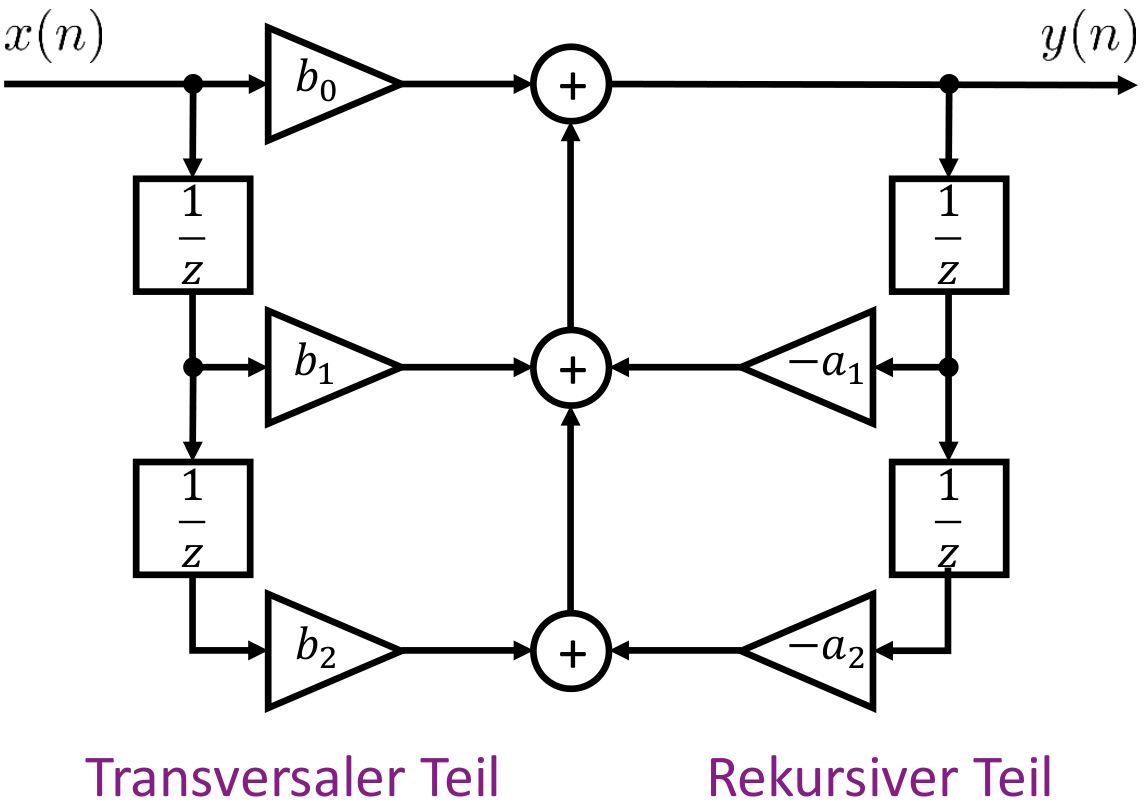
\includegraphics[width=\columnwidth]{Bilder/Signalfluss_plan-graph}
\end{minipage}
\begin{minipage}{0.5\columnwidth}
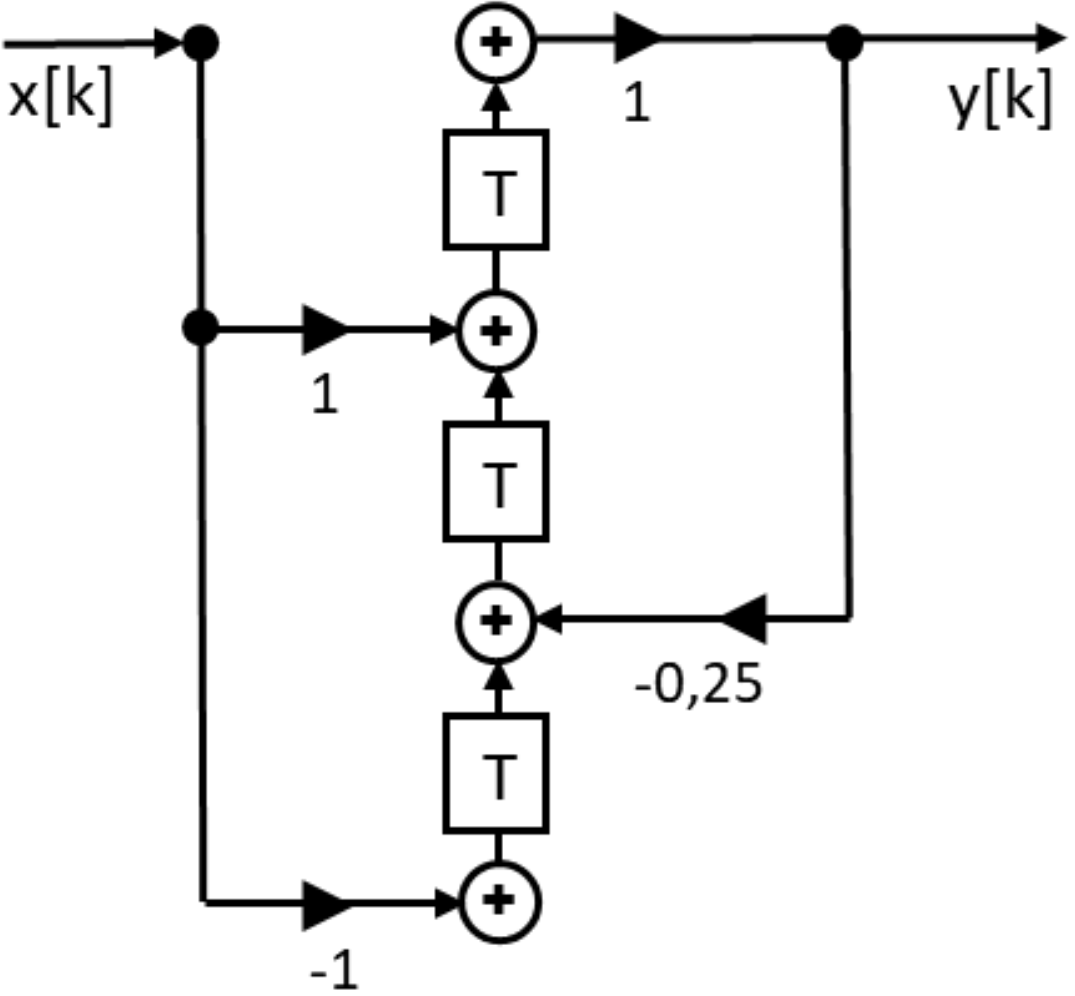
\includegraphics[width=\columnwidth]{Bilder/Signalflussdiagramm}
\end{minipage}

\subsection{Zeitdiskrete Signale im Spektrum}
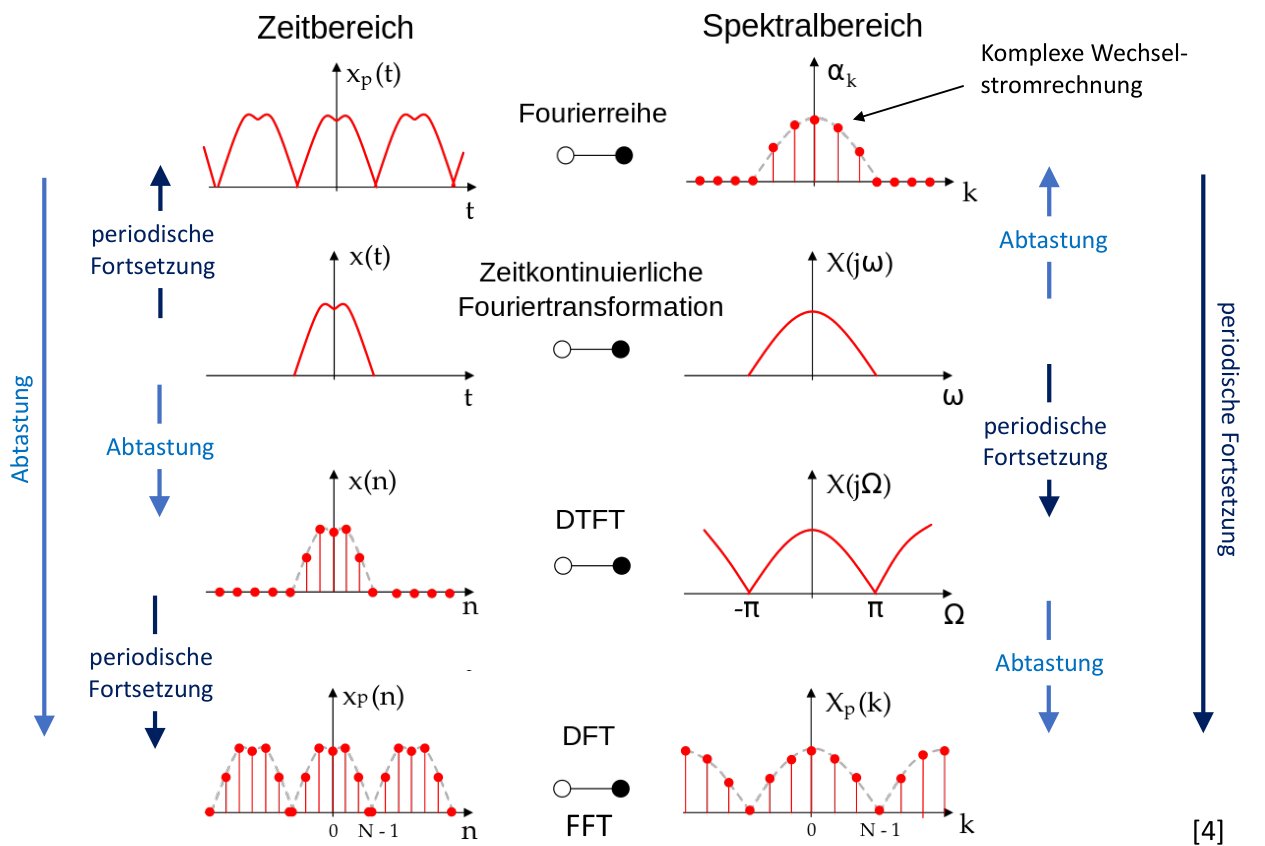
\includegraphics[width=\columnwidth]{Bilder/uebersicht_abtastung_frequenzbereich}
\clearpage
\subsection{Zeitdiskrete Fouriertransformation}
\begin{itemize}
\item zeitdiskrete Fouriertransformation (DTFT):
\[ \boxed{
\underline{X}(\Omega) = \sum_{n=-\infty}^{\infty} x(n) \cdot e^{-j\Omega n}
}
\]
\item Rücktransformation, Synthese:
\[
x(n) = \frac{1}{2\pi}\int_{-\pi}^{\pi} X(\Omega) \cdot  e^{j\Omega n} \, d\Omega
\]
\item Normierte Kreisfrequenz:
\[ \boxed{
\Omega = \omega T = 2\pi f T = 2\pi \frac{f}{f_a} }
\]
{\small Spektrum $\underline{X}(\Omega)$ ist freq.-kontinuierlich und\\ periodisch mit $T=2\pi$. $\rightarrow$ $X(\Omega)=X(\Omega+2\pi)$}
\item Einheit des Spektrums/Signals: $[\underline{X}(\omega)] = x(n)$
\end{itemize}

\subsection{z-Transformation}
Hintransformation, Analysegleichung: 
\[\boxed{
	\underline{X}(z) = \sum_{n=0}^{\infty} x(n) \cdot z^{-n} }
\]
Existiert nur für rechtsseitige (kausale) Folgen/Signale!
\small
\begin{itemize}
	\item Kb darf keine Polstellen enthalten.
	\item Zeitbegrenzte (kausale) Signale: Kb außerhalb\\ des Ursprungs.
	\item Unendlich lange (kausale) Signale: Kb außerhalb\\ des Kreises durch betragsgrößte Polstelle.
\end{itemize}
\normalsize

\subsubsection{Rücktransformation mit PBZ}
Partialbruchzerlegung allgemein:
\[
\underline{X}(z)=\frac{\underline{Z}(z)}{\underline{N}(z)}=\frac{\sum_{m=0}^{M} b_{m} z^{m}}{\sum_{n=0}^{N} a_{n} z^{n}}=\frac{b_{M}}{a_{N}} \cdot \frac{\prod_{m=1}^{M}\left(z-z_{o m}\right)}{\prod_{n=1}^{N}\left(z-z_{x n}\right)}
\]
\textbf{Einfache} Polstellen $p_n$:
\begin{align*}
	\Aboxed{\frac{\underline{X}(z)}{z} & =\frac{c_{0}}{z}+\frac{c_{1}}{z-z_{x 1}}+\frac{c_{2}}{z-z_{x 2}}+\cdots+\frac{c_{N}}{z-z_{x N}}} \\
	\Rightarrow \underline{X}(z) &= c_0 + \sum_{n=1}^{N} c_n \frac{z}{z-p_n} \quad c_0=0, \text{wenn } b_0=0
\end{align*}
Sonderfall: n-fache Polstellen bei z=0:
\begin{align*}
	\underline{X}(z) = \frac{\sum_{m=0}^{M} b_m \cdot  z^m}{a_N \cdot z^N} = \sum_{m=0}^{M} \frac{b_m}{a_N} \cdot z^{m-N}
\end{align*}
\textbf{Mehrfache} Polstellen $p_n$:
\begin{align*}
	\Aboxed{\frac{\underline{X}(z)}{z} &=\frac{c_{0}}{z}+\frac{c_{1}}{z-p_n}+\frac{c_{2}}{\left(z-p_n\right)^{2}}+\cdots+\frac{c_{k}}{\left(z-z_{x n}\right)^{k}}}\\
			\Rightarrow \underline{X}(z) & = c_0 + c_1 \frac{z}{z-p_n}+c_2\frac{z}{(z-p_n)^2}+\cdots+c_k\frac{z}{(z-p_n)^k}
\end{align*}

\subsubsection{Eigenschaften der z-Transformation}
\renewcommand{\arraystretch}{1.7}
{\small 
\begin{tabularx}{\columnwidth}{|c|c|c|}
	\hline
	& $\mathbf{x[n]}$ & \underline{$\mathbf{X}$}$\mathbf{(z)}$\\
	\hline Linearität & $a x_{1}[n]+b x_{2}[n]$ & $a \underline{X}_{1}(z)+b\underline{X}_{2}(z)$ \\
	\hline Verschiebung	& $x[n-k]$ & $z^{-k} \underline{X}(z)$ \\
	\hline Modulation & $a^{n} \, x[n]$ & $\underline{X}\left(\frac{z}{a}\right)$ \\
	\hline Multiplikation & $n \cdot x[n] $ & $-z \frac{d}{d z} \underline{X}(z)$ \\
	\hline Faltung & $x_{1}[n] * x_{2}[n] $ & $ \underline{X}_{1}(z) \cdot \underline{X}_{2}(z)$ \\
	\hline Faltung im BB & $x_{1}[n] \cdot x_{2}[n] $ & $ \frac{1}{2\pi j} \int \underline{X}_1(\eta)\underline{X}_2(\frac{z}{\eta})\frac{1}{\eta}\, d\eta$ \\
	\hline Differenzbildung & $x[n]-x[n-1] $ & $ \frac{z-1}{z} \underline{X}(z)$ \\
	\hline Summenbildung & $\sum_{i=0}^{n} x[i] $ & $ \frac{z}{z-1} \underline{X}(z)$ \\
	\hline
\end{tabularx} }

\subsubsection{Korrespondenzen der z-Transformation}
Normierte Kreisfrequenz $\Omega_1 = \omega T$\\
\renewcommand{\arraystretch}{1.7}
\begin{tabularx}{\columnwidth}{|l|X|X|}
	\hline $\mathbf{N r}$. & $\mathbf{x}[\mathbf{n}]$ & $\mathbf{\underline{X}}(\mathbf{z})$ \\
	\hline 1 & $\delta[n]$ & 1 \\
	\hline 2 & $\delta[n-i]$ & $z^{-i}$ \\
	\hline 3 & $\varepsilon[n]$ & $\frac{z}{z-1}$ \\
	\hline 4 & $\varepsilon[n-i]$ & $\frac{z}{z-1} \cdot z^{-i}$ \\
	\hline \textbf{5} & $n \cdot \varepsilon[n]$ & $\frac{z}{(z-1)^{2}}$ \\
	\hline 6 &  $n^2 \cdot \varepsilon[n]$ & $\frac{z(z+1)}{(z-1)^3}$  \\
\hline 7 & $e^{-a n} \cdot \varepsilon[n]$ & $\frac{z}{z-e^{-a}}$ \\
\hline 8 & $n \, e^{-a n} \cdot \varepsilon[n]$ & $\frac{z e^{-a}}{\left(z-e^{-a}\right)^{2}}$ \\
\hline \textbf{9} & $a^{n} \cdot \varepsilon[n]$ & $\frac{z}{z-a}$ \\
\hline 10 & $a^{n-1} \cdot \varepsilon[n-1]$ & $\frac{1}{z-a}$ \\
\hline \textbf{11} & $n\,a^{n} \cdot \varepsilon[n]$ & $\frac{z a}{(z-a)^{2}}$ \\
\hline 12 & $n \, a^{n-1} \cdot \varepsilon[n]$ & $\frac{z}{(z-a)^{2}}$ \\
\hline 13 & $(n-1) \, a^{n-1} \cdot \varepsilon[n-1]$ & $\frac{1}{(z-a)^{2}}$ \\
\hline 14 & $n^{2} \, a^{n} \varepsilon[n]$ & $\frac{a z(z+a)}{(z-a)^{3}}$ \\
\hline 15 & $\binom{n}{i} a^{n-i} \varepsilon[n-i]$ & $\frac{z}{(z-a)^{i+1}}$ \\
\hline 16 & $\frac{\left(a^{n+1}-b^{n+1}\right)}{a-b} \varepsilon[n] \quad a \neq b$ & $\frac{z^{2}}{(z-a)(z-b)}$ \\
\hline 17 & $\frac{1}{n} \varepsilon[n-1] \cdot \varepsilon[n]$ & $\ln \left(\frac{z}{z-1}\right)$ \\
\hline \textbf{18} & $\sin (\Omega_1 n ) \cdot \varepsilon[n]$ & $\frac{z \sin (\Omega_1)}{z^{2}-2 z \cos (\Omega_1)+1}$ \\
\hline \textbf{19} & $\cos (\Omega_1 n ) \cdot \varepsilon[n]$ & $\frac{z[z-\cos (\Omega_1)]}{z^{2}-2 z \cos (\Omega_1)+1}$ \\
\hline 20 & $a^{n} \sin (\Omega_1 n) \cdot \varepsilon[n]$ & $\frac{z a \sin (\Omega_1)}{z^{2}-2 z a \cos (\Omega_1)+a^{2}}$ \\
\hline 21 & $a^{n} \cos (\Omega_1 n) \cdot \varepsilon[n]$ & $\frac{z[z-a \cos (\Omega_1)]}{z^{2}-2 z a \cos (\Omega_1)+a^{2}}$ \\
\hline 22 & $\operatorname{rect}_{N}[n]$ & $\frac{z-z^{-N}}{z-1}$ \\
\hline
\end{tabularx}
\clearpage

\subsection{LTI-Systeme im Bildbereich}
\subsubsection{Impuls- und Sprungantwort im BB}
$$
	h(n) \, \laplace \, \boxed{\underline{H}(z) = \underline{G}(z) \cdot \frac{z-1}{z} } \qquad \boxed{
	\underline{G}(z) = \underline{H}(z) \cdot \frac{z}{z-1} }
$$




\subsubsection{PN-Diagramm $\Rightarrow$ Frequenzgang}
Wenn zeitdiskretes LTI-System \textbf{stabil}: Ersetze $z=e^{j\Omega}$:\\
\[ \boxed{
	\underline{H}(\Omega)=\left.\underline{H}(z)\right|_{z=e^{j \Omega}} } \quad \text{wenn \textbf{alle} Pole innerhalb des EK.}
\]
\textbf{Ermittlung} $\underline{H}(\Omega)$: Am Einheitskreis des PN-Diagramms \textit{entlang} gegen den UZS für $\Omega > 0$ gehen.\\

$z_o$: Nullstellen, \quad $z_x$: Polstellen
\begin{gather*}
	\underline{H}(z)=\frac{\left(z-z_{o}\right)}{\left(z-z_{x}\right)} \qquad
	\underline{H}(\Omega)=\frac{\left(e^{j \Omega}-z_{o}\right)}{\left(e^{j \Omega}-z_{x}\right)}=\frac{A_{o} e^{j \varphi_{o}}}{A_{x} e^{j \varphi_{x}}}
\end{gather*}
\centering
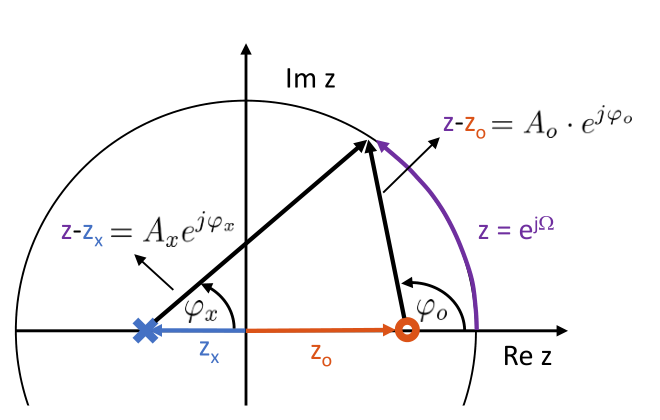
\includegraphics[width=0.7\columnwidth]{Bilder/PN-FreqGang}

\raggedright
\textbf{Betragsfrequenzgang}, Amplitudengang\\
Pole/Nullstellen $\rightarrow$ Amplitude steigt/sinkt.
\[
|\underline{H}(\Omega)| = H(\Omega)=\frac{A_{o}(\Omega)}{A_{x}(\Omega)} = \frac{Y(\Omega)}{X(\Omega)}
\]
\textbf{Phasenfrequenzgang}
\[
\varphi_{H}(\Omega)=\varphi_{o}(\Omega)-\varphi_{x}(\Omega) =\varphi_{Y}(\Omega)-\varphi_{X}(\Omega)
\]

Beispiele:
\makebox[\columnwidth][c]{
	\begin{minipage}{0.5\columnwidth}
		\begin{center}
			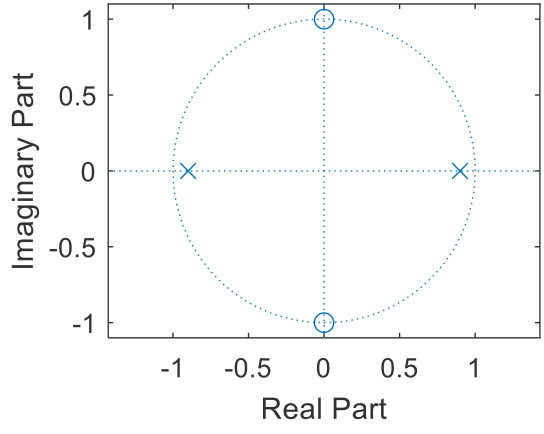
\includegraphics[width=0.9\columnwidth]{Bilder/PN-FreqGang_BSP-P1}
		\end{center}
	\end{minipage}
	\begin{minipage}{0.5\columnwidth}
		\begin{center}
			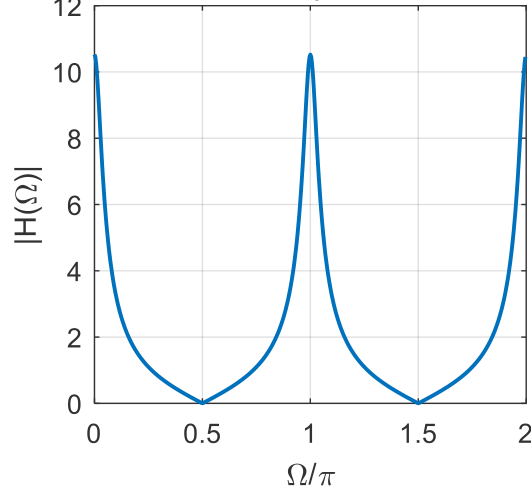
\includegraphics[width=0.8\columnwidth]{Bilder/PN-FreqGang_BSP-P2}
		\end{center}
	\end{minipage}
}
\makebox[\columnwidth][c]{
	\begin{minipage}{0.5\columnwidth}
		\begin{center}
			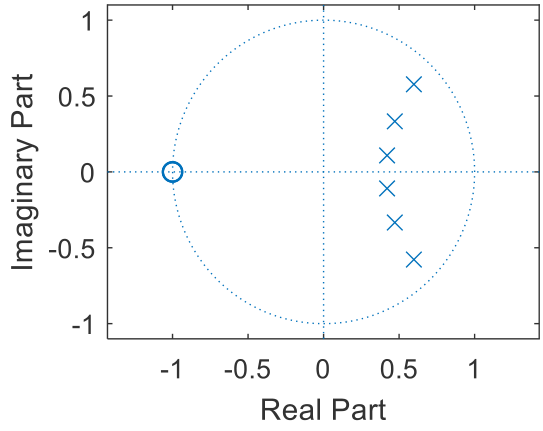
\includegraphics[width=0.9\columnwidth]{Bilder/PN-FreqGang_BSP1-P1}
		\end{center}
	\end{minipage}
	\begin{minipage}{0.5\columnwidth}
		\begin{center}
			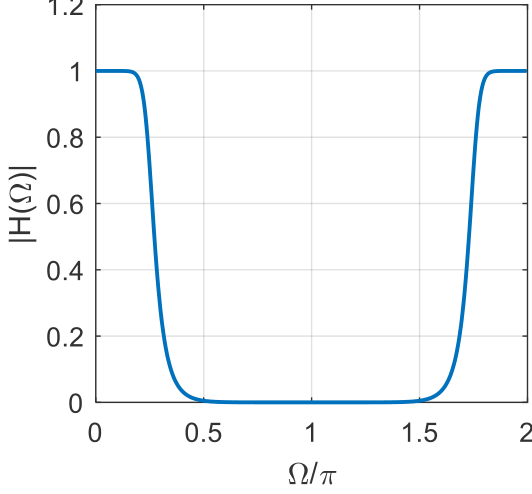
\includegraphics[width=0.8\columnwidth]{Bilder/PN-FreqGang_BSP2-P2}
		\end{center}
	\end{minipage}
}

\subsubsection{Systemantwort auf harm. Eingangssignale}	
LTI-System verändert \textbf{nur} Amplitude und Phase von $x(t)$.\\
Normierte Frequenz $\Omega_1 = \omega T$ bleibt gleich.

\begin{tabular}{cc}
	Gegeben: & $x(n) = \hat{x} \cdot \sin(\Omega_1n+\varphi_x)$\\
	Gesucht: & $y(n) = \hat{y} \cdot \sin(\Omega_1n+\varphi_y)$
\end{tabular}
\begin{gather*}
\boxed{
\hat{y} = \hat{x} \cdot |\underline{H}(\Omega_1)|} \qquad
\boxed{
 \varphi_y = \varphi_x + \varphi_H(\Omega_1) } 
\end{gather*}



%\end{multicols*}
%\subsection{s-Frequenzebene/z-Frequenzebene}
%\begin{center}
%	\begin{tabular}[htpb]{c|c|c}
%		s-Frequenzebene     & $e^{sT} = z$          & z-Frequenzebene     \\
%		\hline
%		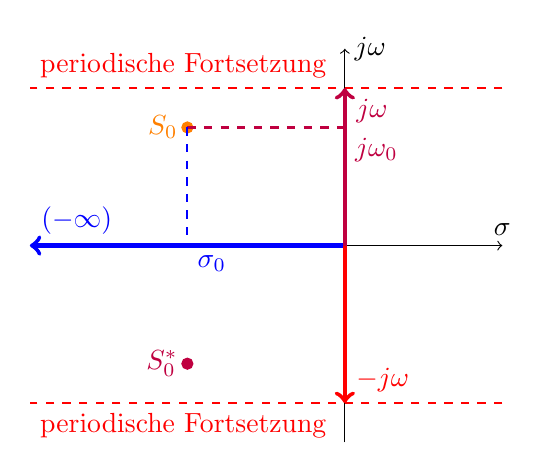
\begin{tikzpicture}[baseline=1]
    \draw[->] (0,-2.5) -- (0,2.5) node[right]{$j\omega$}; %y
    \draw[->] (-4,0) -- (2,0) node[above]{$\sigma$}; %x

    \draw[thick, dashed, red] (2,2) -- (-4,2) node[above right]{periodische Fortsetzung};
    \draw[thick, dashed, red] (2,-2) -- (-4,-2) node[below right]{periodische Fortsetzung};
    \draw[ultra thick, ->, blue] (0,0) -- (-4,0) node[above right]{$(-\infty)$};
    \draw[ultra thick, ->, purple] (0,0) -- (0,2) node[below right]{$j \omega$};
    \draw[ultra thick, ->, red] (0,0) -- (0,-2) node[above right]{$-j \omega$};

    \filldraw[orange] (-2,1.5) circle (2pt) node[left]{$S_0$};
    \draw[thick, dashed, purple] (-2,1.5) -- (0,1.5) node[below right]{$j \omega_0 $};
    \draw[thick, dashed, blue] (-2,1.5) -- (-2,0) node[below right]{$ \sigma_0 $};

    \filldraw[purple] (-2,-1.5) circle (2pt) node[left]{$S_0^*$};
\end{tikzpicture}
 & $\Rightarrow$ & 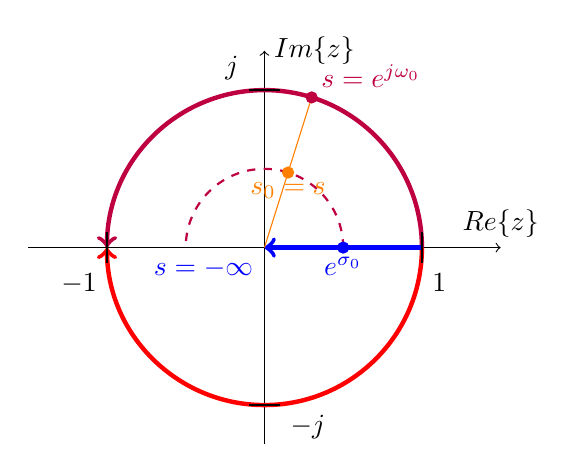
\begin{tikzpicture}[baseline=1]
    \draw[->] (0,-2.5) -- (0,2.5) node[right]{$\mathfrak{Im}\{z\}$}; %y
    \draw[->] (-3,0) -- (3,0) node[above]{$\mathfrak{Re}\{z\}$}; %x

    \draw[thick, color=black, dashed](0,0) circle (2);
    \draw[ultra thick, ->, purple] (2,0) arc (0:180:2);
    \draw[ultra thick, ->, red] (2,0) arc (0:-180:2);
    \draw[ultra thick, ->, blue] (2,0) -- (0,0) node[below left]{$s =-\infty$};

    \draw[thick, dashed, purple] (1,0) arc (0:180:1);

    \draw[thick, black] (0.2,2) -- (-0.2,2) node[above left]{$j$};
    \draw[thick, black] (-0.2,-2) -- (0.2,-2) node[below right]{$-j$};
    \draw[thick, black] (2,0.2) -- (2,-0.2) node[below right]{$1$};
    \draw[thick, black] (-2,0.2) -- (-2,-0.2) node[below left]{$-1$};

    \filldraw[blue] (1,0) circle (2pt) node[below]{$ e^{\sigma_0}$};
    \filldraw[orange] (0.3,0.953) circle (2pt) node[below]{$s_0 = s$};
    \draw[orange] (0,0) -- (0.6,1.907) {};
    \filldraw[purple] (0.6,1.907) circle (2pt) node[above right]{$s=e^{j \omega_0}$};
\end{tikzpicture}
 \\
%	\end{tabular}
%\end{center}
%\begin{multicols*}{2}
%\subsection{s-Frequenzebene/z-Frequenzebene}

\subsubsection{Klassifizierung von Systemen}
% Die mathematischen Beschreibung fehlen. wurden nie gebraucht während lernen. Kap6S63 6.5.7
\begin{itemize}[leftmargin=*]
	\item \textbf{Transversale Systeme}, FIR, AR:
	
	{\small Finite Impulse Response (FIR), Auto-Regressive (AR)\\
		Keine Rückführung von Ausgang $y(n)$ auf Eingang $x(n)$.}\\
	$\Rightarrow$ $a_k=0 \texttt{ für } k>0$.\\
	$\Rightarrow$ Alle Pole liegen im Ursprung.
	
	\makebox[\columnwidth][c]{
		\begin{minipage}{0.5\columnwidth}
			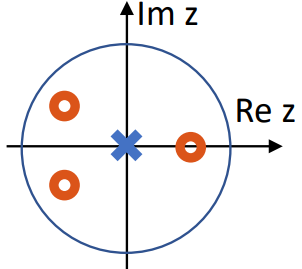
\includegraphics[width=0.7\columnwidth]{Bilder/Transversale_Systeme_}
		\end{minipage}
		\hspace{-1em}
		\begin{minipage}{0.5\columnwidth}
			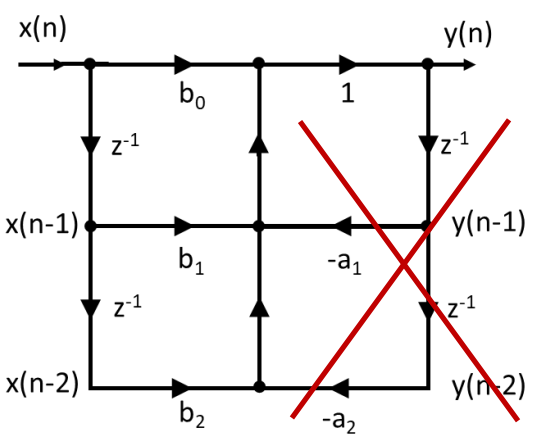
\includegraphics[width=0.8\columnwidth]{Bilder/Transversale_Systeme_SG}
		\end{minipage}
	}
	
	\item \textbf{Rekursive Systeme}, IIR, MA:
	
	{\small Infinite Impulse Response (IIR), Moving-Average (AR)\\
		Aktueller Ausgangswert hängt nur vom aktuellen Eingangswert
		und früheren Ausgangswerten ab.}\\
	$\Rightarrow$ $b_k=0 \texttt{ für } k>0$.\\
	$\Rightarrow$ Alle Nullstellen liegen im Ursprung.
	
	\makebox[\columnwidth][c]{
		\begin{minipage}{0.5\columnwidth}
			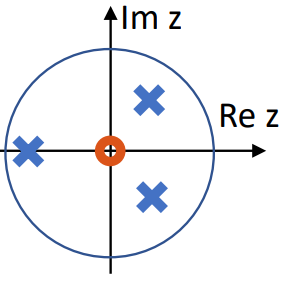
\includegraphics[width=0.7\columnwidth]{Bilder/Rekursive_Systeme}
		\end{minipage}
		\hspace{-1em}
		\begin{minipage}{0.5\columnwidth}
			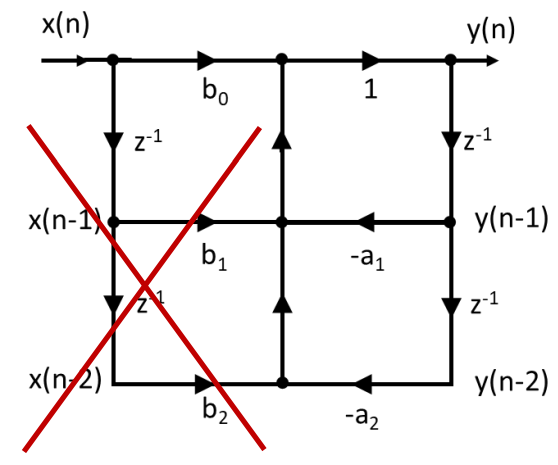
\includegraphics[width=0.8\columnwidth]{Bilder/Rekursive_Systeme_SG}
		\end{minipage}
	}
	\item ARMA: Auto-Regressive Moving Average\\ $\rightarrow$ transversal-rekursives System.
\end{itemize}
